
%%%%%%%%%%%%%%%%%%%%%%% file typeinst.tex %%%%%%%%%%%%%%%%%%%%%%%%%
%
% This is the LaTeX source for the instructions to authors using
% the LaTeX document class 'llncs.cls' for contributions to
% the Lecture Notes in Computer Sciences series.
% http://www.springer.com/lncs       Springer Heidelberg 2006/05/04
%
% It may be used as a template for your own input - copy it
% to a new file with a new name and use it as the basis
% for your article.
%
% NB: the document class 'llncs' has its own and detailed documentation, see
% ftp://ftp.springer.de/data/pubftp/pub/tex/latex/llncs/latex2e/llncsdoc.pdf
%
%%%%%%%%%%%%%%%%%%%%%%%%%%%%%%%%%%%%%%%%%%%%%%%%%%%%%%%%%%%%%%%%%%%


\documentclass[runningheads,a4paper]{llncs}

\usepackage{amssymb}
\setcounter{tocdepth}{3}
\usepackage{graphicx}


\usepackage{listings}
\usepackage{upquote}
\usepackage{paralist}
\usepackage{commath}
\usepackage{enumerate}
%\usepackage[cmex10]{amsmath}
%\usepackage[pdftex]{graphicx}
\usepackage{amssymb}
\usepackage[caption=false,font=footnotesize]{subfig}

\usepackage{url}
\urldef{\mailsa}\path|{mohamed.abbadi, francesco.digiacomo, cortesi}@unive.it|
\urldef{\mailsb}\path|p.spronck@uvt.nl|
\urldef{\mailsc}\path|{costg,maggg}@hr.nl|
\newcommand{\keywords}[1]{\par\addvspace\baselineskip
\noindent\keywordname\enspace\ignorespaces#1}

\begin{document}

\mainmatter  % start of an individual contribution

% first the title is needed
\title{Casanova: A simple, high-performance language for game development}

% a short form should be given in case it is too long for the running head
\titlerunning{Casanova: A simple, high-performance language for game development}

% the name(s) of the author(s) follow(s) next
%
% NB: Chinese authors should write their first names(s) in front of
% their surnames. This ensures that the names appear correctly in
% the running heads and the author index.
%
\author{Mohamed Abbadi, Francesco Di Giacomo, Agostino Cortesi\\Pieter Spronck, Giulia Costantini, Giuseppe Maggiore}
%
\authorrunning{Mohamed Abbadi, Francesco Di Giacomo, Agostino Cortesi\\Pieter Spronck, Giulia Costantini, Giuseppe Maggiore}
% (feature abused for this document to repeat the title also on left hand pages)

% the affiliations are given next; don't give your e-mail address
% unless you accept that it will be published
\institute{Universit\`a Ca' Foscari DAIS, Venice, Italy\\
Tilburg University, Tilburg, Netherlands\\
Hogeschool Rotterdam, Rotterdam, Netherlands\\
\mailsa\\
\mailsb\\
\mailsc\\
\url{http://casanova.codeplex.com/}}

%
% NB: a more complex sample for affiliations and the mapping to the
% corresponding authors can be found in the file "llncs.dem"
% (search for the string "\mainmatter" where a contribution starts).
% "llncs.dem" accompanies the document class "llncs.cls".
%

\maketitle



\begin{abstract}
In many Real-Time Strategy (RTS) games, players develop an army in real time, then attempt to take out one or more opponents. Despite the existence of basic similarities among the many different RTS games, engines of these games are often built ad hoc, and code re-use among different titles is minimal. We created a design pattern called ``Resource Entity Action'' (REA) that abstracts the basic interactions that entities have with each other in most RTS games. This paper discusses the REA pattern and its language abstraction. We also discuss the implementation in the Casanova game programming language. Our analysis shows that the pattern forms a solid basis for a playable RTS game, and that it achieves considerable gains in terms of lines of code and runtime efficiency. We conclude that the REA pattern is a suitable approach to the implementation of many RTS games. 
\end{abstract}

\lstset{
    tabsize=2,
        upquote=true,
        basicstyle=\scriptsize,
        columns=fixed,
        showstringspaces=false,
        mathescape,
        frame=single,
        showtabs=false,
        showspaces=false,
        showstringspaces=false,
        identifierstyle=\ttfamily,
        keywordstyle=\ttfamily
}


%Introduction
\section{Introduction}
\label{sec:introduction}
%%%%%%%%%%%%%%%%%%%%%%%%%%%%%%%%%%%%%%%%%%%%%%%%%%%%%%%%%%
% intro.tex
%%%%%%%%%%%%%%%%%%%%%%%%%%%%%%%%%%%%%%%%%%%%%%%%%%%%%%%%%%

Game are:
- complex
- require performance

Low-level languages do not cut it fully.

We will:
(A) discuss game constraints
  - discuss traditional approaches and their limitations
  - discuss similarities between game genres and try and find a general framework
  - define a language that is built around this general framework, and which makes it easy
  - reason on why we'd rather have a new language and not just a library
  - give syntax, typing, semantics
(B) give optimization transformations of the language
(C) give a detailed case study
  - give benchmarks that show how effective our optimizations are and how they are completely automated (they require no effort on the part of the programmer)


%Problem Statement
\section{Technical challenges in games development}
\label{sec:problem statement}
In this section we discuss games and their complexity through a case study. We consider a sample which fits within the space constraints of a paper, which at the same time shows the complex interactions that are typical for games.

\subsection{Running example}
The running example we use is a patrol moving through checkpoints. The state of the patrol is made up by the position of the patrol \texttt{P}, and its velocity \texttt{V}.
\begin{lstlisting}
P is a 2D Vector
V is a 2D Vector
Checkpoints is a list of 2D Vectors
\end{lstlisting}
The logic of the game is given using a pseudo language:
\begin{lstlisting}
P is integrated by V over dt
V points towards the next checkpoint until
  the checkpoint is reached, then becomes
  zero for ten seconds (the patrol is idle)
\end{lstlisting}

A game is said to run as a sequence of time slices, called ``frames.'' A typical game runs at 30 to 60 frames per second. The pseudo code above describes the logic of the patrol, which runs every frame. The logic shows a typical dynamic present in any game, which is made up by continuous components (the update of \texttt{P} in our case) and discrete components (the update of \texttt{V}). As a result, \texttt{P} changes every frame, while \texttt{V} only changes upon reaching a checkpoint.

\subsection{Common issues}
Dynamics such as the one described above are built in games either with engines or by hand.
\paragraph{Engines} An engine is a library built to offer solutions for specific tasks (such as graphics and physics control) in order to speed up the development process, by promoting code reuse and reducing mistakes. By hiding complexity inside libraries and editors, developers only need to adapt their design to the engine. While popular, engines tend to have significant issues:
\begin{itemize}
\item Engines are often difficult, or even impossible, to expand and to adapt to the needs of the developer using them; this limits developers because some aspects of design might need to be adapted or left out due to of lack of specific support by the engine;
\item Engines are often closed libraries. Even though engines are internally optimized, the possibilities for global optimization that take into account the game structure are very limited;
\item Expertise is needed to master an engine. Since most (if not all) engines are highly complex to use, a significant effort of the developers is spent on learning the intricacies of the engine.
\end{itemize}
In general, a good engine offers good performance and a reduced possibility to make mistakes, but at the same time limits developers to the engine features and asks them to master most features before using the full capabilities of the engine.

\paragraph{Hand made implementations} A hand made implementation is used when developers are looking for specific behaviors, want to have more control on the game implementation, or when the support of the underlying platform is poor.
Hand made implementations raise important issues to be considered before starting a new project:
\begin{itemize}
\item Games tend to be very large applications. As size increases, the number of interactions increases as well, together with the possibility to make mistakes;
\item Optimization (when done by hand) adds complexity, because it requires supplementary data structures and may change the implementation of the game interaction. Optimization may also lead to (\textit{i}) implementation issues (for instance some optimization may work only on specific architectures), and (\textit{ii}) maintainability issues (any change in the game design should keep into account its repercussions on the implementation).
\end{itemize}


We now present an example of hand-made implementation of the patrolling dynamics following the style of \cite{millington2009artificial}:
\begin{lstlisting}
class Patrol:
  enum State:
   MOVING
   STOP

  public P, V, Checkpoints
  private myState, currentCheckpoint, timeLeft

  def loop(dt):
   P = P + V * dt
   if myState == MOVING:
     if P == Checkpoints[currentCheckpoint]:
       myState = STOP
       V = Vector2.Zero
       timeLeft = 10
   elif myState == STOP:
     if timeLeft < 0:
       currentCheckpoint += 1
       currentCheckpoint %= Checkpoints.length
       myState = MOVING
       V = Normalize(
            Checkpoints[currentCheckpoint] - P))
     else
       timeLeft -= dt
\end{lstlisting}
The \texttt{loop} function implements the patrolling behavior. It takes one argument \texttt{dt} which represents the delta time elapsed since the last frame. The very first line of the \texttt{loop} body implements the position update behavior. The velocity behavior depends on whether the patrol is moving or idle. While moving, we stop the patrol as soon as he reaches the checkpoint, and set the wait timer to 10 seconds. If the patrol is idle and the countdown is elapsed, the next checkpoint is selected. At this point the patrol points toward the new checkpoint and starts moving again.


% In general, solutions made by hand are desirable when building anything that is not readily supported by existing libraries or engines.

\subsection{Discussion}
The patrolling sample illustrates a common division between design and implementation in games. Deceptively simple problem descriptions turn out to require surprisingly articulated implementations. Complexity mainly originates from the explicit definition and management of a series of \textit{spurious variables} that are needed to program the logical flow of the problem but which do not come up in the design. In our case study, the spurious variables are \texttt{myState} (together with the definition of the state structure) and \texttt{timeLeft}.

A language suited for game development by persons for whom game development is not their main job, has two main requirements:
\begin{itemize}
\item \textit{Performance}: games are highly interactive applications which tend to be filled with many dynamic elements; if the language in which they are built does not guarantee high performance, the player experience will suffer;
\item \textit{Simplicity}: the language should be easy to understand and easy to express game functionality in; if the language is not simple in these respects, it requires an amount of training that is not within reach of those who are not game developers by profession.
\end{itemize}

Below we introduce a game-centered programming language and show how to rebuild the sample above with fewer spurious constructs, in a way that is closer to a higher-level, readable description. 


%Orch model
%\section{A concurrency model for games}
%\label{sec:orch model}
%In this section we discuss a model for computation which was directly inspired by the ``orchestration model'' \cite{misra2007computation}, and we show how this model simplifies the example above.

\subsection{Our model}
We begin with the observation that components can be treated as independent and concurrent programs.
Our model is tiny since it consists of four operators:  (\texttt{$\rightarrow$}) the bind operator, (\texttt{||}) the parallel operator, (\texttt{$\downarrow$}) the yield operator, and (\texttt{let}) the expression definition operator.

Given two concurrent programs, \texttt{g} and \texttt{f}: \texttt{f$\rightarrow$g} runs \texttt{g} after \texttt{f} has terminated. The expression becomes \texttt{f>g} if we do not want any result of \texttt{f} to enter in the scope of \texttt{g}); \texttt{(f||g)} runs \texttt{f} and \texttt{g} in parallel. \texttt{$\downarrow x$, v} changes the value of v into x (x is a variable defined either as an argument of the current function or a variable defined outside the function itself); \texttt{let} allows the assignment of expressions to labels in the form of \texttt{let name = expr}. The \textit{state} is made up from the definition of all the variables involved in the logic.


\subsection{Re-implementation of the case study}
We now show how our model can express the dynamic of a game by using it to re-write our case study. 
The implementation is divided into three blocks:
\begin{enumerate}
\item \texttt{UPDATE}, implements the logic ;
\item \texttt{DRAW}, draws the entities of the game; 
\item \texttt{GAME}, coordinates the execution of both \texttt{UPDATE} and \texttt{DRAW}.
\end{enumerate}

The new implementation of the game is now given:
In the \texttt{UPDATE} block we define the underlying logic of the game. The key pressure is caught by \texttt{WaitSpacePressed} which waits until the \texttt{space} key is first pressed and then released. The logic of the light switch waits until the space key is pressed, and once this event occurs it turns \texttt{on} the light switch. We turn back to \texttt{off} when we press again the space button. Afterwards, it recurses.
\begin{lstlisting}[caption=LOGIC]
let WaitSpacePressed = 
  wait (Keyboard.Down(Space)) $\rightarrow$
  wait (Keyboard.Up(Space))
let Update sprite_color tick_status = 
  WaitSpacePressed $\rightarrow$
  $\downarrow$ tick_status, Status.Play $\rightarrow$
  $\downarrow$ sprite_color Color.White $\rightarrow$  
  WaitSpacePressed $\rightarrow$
  $\downarrow$ tick_status, Status.Play $\rightarrow$
  $\downarrow$ sprite_color Color.Black $\rightarrow$
  Update sprite_color tick_status
\end{lstlisting}
The \texttt{DRAW} block draws the light switch (which is called \texttt{sprite}) and then recurs.
\begin{lstlisting}[frame=single, caption=DRAW]
let Draw sprite = DrawSprite sprite $\rightarrow$ Draw
\end{lstlisting}
The \texttt{GAME} block loads the light switch sprite (setting its initial color to \texttt{Black}), and runs \texttt{UPDATE} and \texttt{DRAW} in parallel.
\begin{lstlisting}[frame=single, caption=LOOP]]
let sprite = LoadSprite "mySprite.png"
let sound = LoadSoundManager()
let Game = Update(sprite.Color, sound.Status) || 
           Draw(sprite)				
\end{lstlisting}
The spurious constructs used to maintain the state machine are no longer present explicitly, but stored and handled implicitly in the form of \textit{program counters} of the various processes. This is due to the control flow semantics of our model. The resulting program has more in common (from the perspective of readability) with the \textit{definition} of the light switch problem than the program presented in Section 2.


We will now proceed with the definition of the Casanova 2 programming language that is inspired by the concepts of orchestration languages. 

%Casanova 2
\section{Casanova 2}
\label{sec:casanova 2}
Languages, in general, offer more expressive power than engines, because of the possibility to combine and nest the constructs. A language specifically designed and built with game programming in mind can help with common aspects of game development (such as time, concurrency, and state updates) that regular languages do not encompass.
In this regard, we present the language Casanova 2, based on \cite{maggiore2012designing}, which takes its inspiration from the orchestration model of \cite{misra2007computation}. We show how Casanova 2 is designed in particular to express the typical dynamics present in games.

\subsection{The basic idea behind Casanova 2}
An abstraction of a game should be able to represent its main elements, i.e., its state variables and their (discrete and dynamic) interactions.
For this purpose, we built an (intentionally) small programming language of which the main features are \textit{state} and \textit{rules}:
\begin{enumerate}[\itshape(i)]
\item The \textit{state} of a game is represented by a hierarchical type definition. Each node of the hierarchy is called an \textit{entity} (besides the root, which is called \textit{world}). Each entity contains a series of fields that represent primitive types, collections, or even references to other entities. Through access to shared data entities we achieve concurrent coordination.
\item The logic of each entity is defined as a series of implicitly parallel looping code blocks. Each implicit block, called a \textit{rule}, represents a specific dynamic of the entity. A rule represents a dynamic, which can be continuous (simple and effect-free) or discrete (with side-effect, the most important of which is \textit{wait}).
\end{enumerate}
\subsection{Casanova patrol}
We now show how we rewrite the patrol program presented in Section \ref{sec:problem statement} using Casanova 2.
\begin{lstlisting}[caption=Patrol in Casanova 2]
world Patrol = {
   V : Vector2
   P : Vector2
   Checkpoints : [Vector2]

   rule P = P + V * dt

   rule V =
    for checkpoint in Checkpoints do
      yield $\norm{\texttt{checkpoint - P}}$
      wait P = checkpoint
      yield Vector2.Zero
      wait 10<s>
}
\end{lstlisting}

The first three lines within the definition of Patrol describe the game state, containing three variables: the velocity \texttt{V}, the position \texttt{P}, and a checkpoint list \texttt{Checkpoints}. The next line gives the continuous dynamic, namely the rule P which runs once per frame, i.e., at every frame the position \texttt{P} is integrated by the velocity \texttt{V} over \texttt{dt} (a global value supplied by the system that represents the time difference between the current and the previous frame). The remainder of the definition gives the discrete dynamic, namely the rule V, which represents the movement between checkpoints. The checkpoints are traversed in order, and for each selected checkpoint \texttt{checkpoint} we change the value of the velocity in order to move the patrol towards it (\texttt{yield checkpoint - P}). Then, we wait until the patrol reaches the checkpoint (\texttt{wait P = checkpoint}), and once the checkpoint is reached we stop the patrol, by setting its velocity to 0 (\texttt{yield Vector2.Zero}) for 10 seconds (\texttt{wait 10<s>}). At this point the loop continues and a new checkpoint is selected. We reiterate the list again once we have traversed all the checkpoints.

Note that, in general, a game can be considered a series of entities that run in synchronization in order to achieve a specific goal. In Casanova 2 every entity in the state (as well as every rule in an entity) is in essence an \textit{independent} concurrent program \cite{schneider1997concurrent}. Coordination between these programs happens through a shared state.


%Consider the following, based on the Boids algorithm \cite{reynolds1987flocks}, where a group of subordinates are synchronized in order to follow a leader (whose behavior is the same as the patrol presented above).
%\begin{lstlisting} [caption=Boids in Casanova 2]
%entity Subordinate = {
%   Leader   : Patrol
%   Group    : [Subordinate]
%   MaxSpeed : Vector2
%   P : Vector2
%   V : Vector2
%   rule P = P + V * dt
%   rule V =
%    let repulsion =
%       [for p in Group do
%        sumBy Normalize$(\texttt{P} - \texttt{p.P}) * (1 - \sigma(d(\texttt{P}, \texttt{p.P})))$]
%    yield (Normalize$(\texttt{Leader.P} - \texttt{P})$ +
%           Normalize$(\texttt{repulsion})) * \texttt{MaxSpeed}$
%}
%\end{lstlisting}\footnote{$\sigma$ is a sigmoid function, $d$ represents a distance function}

%During execution each subordinate follows the leader, avoiding at the same time collisions with his team-mates.
%This behavior requires synchronization, which is achieved by the rule on the velocity \texttt{V}. We distinguish the leader (\texttt{Leader} of type \texttt{Patrol}) from the group (\texttt{Group} of type \texttt{[Subordinate]}): their behaviors are different, so their rules must be different as well. Given a subordinate, at every iteration we update its position \texttt{P} (by integrating \texttt{P} by \texttt{V} over \texttt{dt}) and its velocity \texttt{V} (computing a repulsion value to try to avoid collisions with other members of the group, and then reducing the gap between the selected subordinate and the leader).

% PS: I do not really understand what this subsubsection is trying to argue. Please make that clear.


\subsection{Syntax}
The syntax of the language (here presented in Backus-Naur form \cite{strings2010backus}) is rather brief. It allows the declaration of entities as simple functional types (records, tuples, lists, or unions). Records may have fields. Rules contain expressions which have the typical shape of functional expressions, augmented with \texttt{wait}, \texttt{yield}, and queries on lists:
\begin{lstlisting}[caption=Casanova 2 syntax]
<Program> ::=
    <moduleStatement> {<openStatement>}
    <worldDecl> {<entityDecl>}

<moduleStatement> ::= module id
<openStatemnt>    ::= open id
<worldDecl>    ::= world id ["("<formals>")"] =
                   <worldOrEntityDecl>
<entityDecl>   ::= entity id ["("<formals>")"] =
                   <worldOrEntityDecl>
<worldOrEntityDecl> ::= "{" <entityBlock> "}"
<entityBlock>  ::= {<fieldDecl>} {<ruleDecl>}
                   <create>
<create> ::= Create "(" {<formals>} ") = <expr>
<formals>   ::= id [":" <type>] {"," <formals>}
<fieldDecl> ::= id [":" <type>]
<ruleDecl>  ::= rule id {"," id} "=" <expr>
<type>      ::= int |boolean  |float |Vector2
                |Vector3 |string |char
                |list "<" <type> ">" |<generic>
                |<type> "[" "]" |id
<generic>     ::= "'" id
<expr> ::= ...(* typical expressions : let, if,
                 for , while , new, etc. *)
           | wait (<arithExpr> | <boolExpr>)
           | yield | <arithExpr> | <boolExpr>
           | <literal> | <queryExpr> | <seq>
<seq>        ::= <expr> <expr>
<arithExpr>  ::= ...//arithmetic expressions
<boolExpr>   ::= ...//boolean expressions
<literal>    ::= ...//strings , numbers
<queryExpr>  ::= ...//query expressions
\end{lstlisting}


\subsection{Semantics}
The semantics of Casanova 2 is \textit{rewrite-based} \cite{klop1990term}, meaning that the current game world is transformed into another one with different values for its fields and different expressions for its rules.
Given a game world $\omega$, the world is structured as a tree of entities. Each entity $E$ has some fields $f_1 \dots f_n$ and some rules $r_1 \dots r_m$.
\begin{lstlisting}[mathescape]
E = { Field$_1$ = f$_1$; $\dots$; Field$_n$ = f$_n$;
      Rule$_1$ = r$_1$; $\dots$; Rule$_m$ = r$_m$ }
\end{lstlisting}
Each rule acts on a subset of the fields of the entity by defining their new value after one (or more) ticks of the simulation. For simplicity, in the following we assume that each rule updates all fields simultaneously.


An entity is updated by evaluating, in order, all the rules for the fields:
\begin{lstlisting}[mathescape]
tick(e:E, dt) =
 { Field$_1$=tick(f$_1^m$, dt); $\dots$; Field$_n$=tick(f$_n^m$, dt);
   Rule$_1$=r$_1'$; $\dots$; Rule$_m$=r$_m'$ }
where
  f$_1^m$, $\dots$, f$_n^m$, r$_m'$ = step(f$_1^{m-1}$, $\dots$, f$_n^{m-1}$, r$_m$)
  .
  .
  f$_1^1$, $\dots$, f$_n^1$, r$_1'$ = step(f$_1$, $\dots$, f$_n$, r$_1$)
\end{lstlisting}
We define the \texttt{step} function as a function that recursively evaluates the body of a rule. The function evaluates expressions in sequential order until it encounters either a \texttt{wait} or a \texttt{yield} statement. It also returns \textit{the remainder of the rule body}, so that the rule will effectively be resumed where it left off at the next evaluation of \texttt{step}:
\begin{lstlisting}[mathescape]
step(f$_1$, $\dots$, f$_n$, {let x = y in r$'$}) =
  step(f$_1$, $\dots$, f$_n$, r$'$[x:=y])

step(f$_1$, $\dots$, f$_n$, {if x then r$'$ else r$''$; r$'''$})
  when (x = true) = step(f$_1$, $\dots$, f$_n$, {r$'$; r$'''$})

step(f$_1$, $\dots$, f$_n$, {if x then r$'$ else r$''$; r$'''$})
  when (x = false) = step(f$_1$, $\dots$, f$_n$, {r$''$; r$'''$})

step(f$_1$, $\dots$, f$_n$, {yield x; r$'$}) = x, r$'$

step(f$_1$, $\dots$, f$_n$, {wait n; r$'$})
  when (n > 0.0) = f$_1$, $\dots$, f$_n$, {wait (n-dt); r$'$}

step(f$_1$, $\dots$, f$_n$, {wait n; r$'$})
  when (n = 0.0) = step(f$_1$, $\dots$, f$_n$, r$'$)

step(f$_1$, $\dots$, f$_n$, {for x in y:ys do r$'$; r$''$})
  step(f$_1$, $\dots$, f$_n$,
       {r$'$[x:=y];
        for x in ys do r$'$; r$''$})

step(f$_1$, $\dots$, f$_n$, {for x in [] do r$'$; r$''$})
  step(f$_1$, $\dots$, f$_n$, r$''$)
\end{lstlisting}

\subsection{Compiler description}
Specific syntax built around the concept of altering the execution flow of a Casanova program allows the Casanova compiler to translate a Casanova program into an equivalent and high performance low-level program with the same semantics. The result is a high performance program made by a single switch structure, without nesting.
A big advantage of this solution is that we may ignore typical software engineering rules, such as readability and code maintainability (as readability and maintainability are only needed for the Casanova specification of the game).

Usually, software engineering implementations are based on a series of nested state machines, but nesting yields a low performance because of the state selection. In contrast, the Casanova compiler produces an inlining of all the nested state machines into a single sound and fast state machine (which code is pretty much unreadable).
% The correct choice of constructs in a Casanova program is fundamental in order to allow the compiler to apply the appropriate transformations. Coding the state machines into Casanova is possible by hand, although difficult as the game increases in terms of dynamics (a series of nested \texttt{if} that mimic the decisions), but no guarantees about correctness and performance can be provided by our tool.





%Evaluation
\section{Evaluation}
\label{sec:evaluation}
We now present an RTS game we used as a case study, created with Casanova, and the benchmarks that test the action implementation. In the game players must conquer a star system made up of various planets. Each planet builds fleets which are used to fight the fleets of the other players and to conquer more planets. A planet is conquered when a fleet of a player is near it and no other enemy fleet is defending it.

\subsection{Case study}

Three actions are required in this game: The first action, called \texttt{Fight Action}, defines how a fleet fights enemy fleets in range. The fight action subtracts $0.5 \cdot dt$ \texttt{life} points from the in-range enemy fleet during every frame (action tick).

\begin{lstlisting}[language=Caml]
Fleet = {Position: Rule Vector2;FightAction: FightAction;Owner: Ref Player;Life: Var float32;Fight: FightAction }
\end{lstlisting}

The Fight Action is defined as follows:

\begin{lstlisting}[language=sql]
FightAction = TARGET Fleet; RESTRICTION Owner <> Owner; RADIUS 150.0; TRANSFER CONSTANT Life - 0.5;
\end{lstlisting}

The target is an entity of which the type is \textbf{Fleet}. The condition to execute the action is that the fleet must be an enemy (i.e., not the player). The \texttt{attack range} is 150 units of distance. 0.5 \texttt{life} points are subtracted for every attack.

The second action is called \texttt{BuildAction}. It allows a planet to create a ship. In order to build a ship, a planet must gather 10 mineral units. Each planet has a field called \texttt{GatherSpeed} which determines how fast it gathers minerals. Every tick the planet's mineral stash is increased by this amount. This action is a threshold action where the threshold value is the minerals of the planet. As soon as the threshold value is reached, we set the field \texttt{NewFleet} to TRUE (it is used by the engine to create a new fleet), and \texttt{Minerals} to 0 to reset the counter. The planet and its actions are:

\begin{lstlisting}[language=Caml]
Planet = {Position: Vector2;Owner: Rule Ref Player;NewFleet: Rule bool;BuildAction:BuildAction;EnemyOrbitingFleetsAction : EnemyOrbitingFleetsAction;GatherSpeed: float32;Minerals: Var float32 }
\end{lstlisting}

\begin{lstlisting}[language=sql]
BuildAction =
TARGET Self; TRANSFER CONSTANT Minerals + GatherSpeed; THRESHOLD Minerals 10.0; OUTPUT NewFleet := true; OUTPUT Minerals := 0.0
\end{lstlisting}

A Casanova rule is appointed to read the value of NewFleet and, when it is true, to spawn a new fleet.

The third action is required to check if a planet can be conquered by a fleet. A fleet can conquer a planet if there is no enemy fleet near it and if it is sufficiently close. Thus the action definition is the following:

\begin{lstlisting}[language=sql]
EnemyOrbitingFleetsAction =
TARGET Fleet; RESTRICTION Owner Not Eq Owner; RADIUS 25.0; INSERT Owner -> EnemyOrbitingFleets
\end{lstlisting}

The action will add an enemy fleet close enough to change the owner of the planet.

%Even the concept of drawing lasers can be implemented using the INSERT clause simply adding it to \texttt{FightAction} which inserts in a list all the targeted ships positions. In this way we can draw a laser from the source position to the target position. We omit this aspect for brevity.

\subsection{Evaluation}

We evaluated the performance of our approach with the case study, and two extra examples: an asteroid shooter, and an expanded version of the case study with more complex rules. All were implemented in Casanova. Table \ref{tab:code_length} shows a code length comparison between the REA implementation and standard Casanova rules for all three.

We note that in games with basic dynamics the code saving is low, due to the fact that there are few repeated patterns. The advantage of using REA becomes evident in a game with actions involving many types of targets, such as the expanded case study. Furthermore, we managed to drastically increase the performance of the game logic: as Figure \ref{fps_chart} shows, using REA (labeled ``with actions'') results in a speedup factor of 6 to 25, due to automated optimizations in the query evaluation. We also note that our implementation is flexible and general since it is possible to use actions to express a behaviour, such as a projectile collision, which is outside the domain of RTS games and traditional resource-based systems.

\begin{table}
\centering
\caption{CS (case study), Asteroid Shooter and Expanded CS code length}
\label{tab:code_length}
\begin{tabular}
{|l|c|c|c|c|c|c|}
\hline
& Game Entities & Rules & Actions & Total\\
\hline
\textit{CS with REA} & 41 & 71 & 19 & 131\\
\hline
\textit{CS without REA} & 40 & 90 & 0 & 130\\
\hline
\textit{Asteroid shooter with REA} & 33 & 33 & 6 & 72\\
\hline
\textit{Asteroid Shooter without REA} & 34 & 44 & 0 & 78\\
\hline
\textit{Extended CS with REA} & 135 & 138 & 40 & 313\\
\hline
\textit{Extended CS without REA} & 135 & 328 & 0 & 463\\
\hline
\end{tabular}
\end{table}
\begin{figure}
\centering
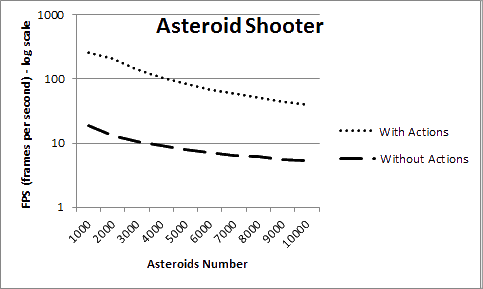
\includegraphics[scale=0.7]{Shooter.png}
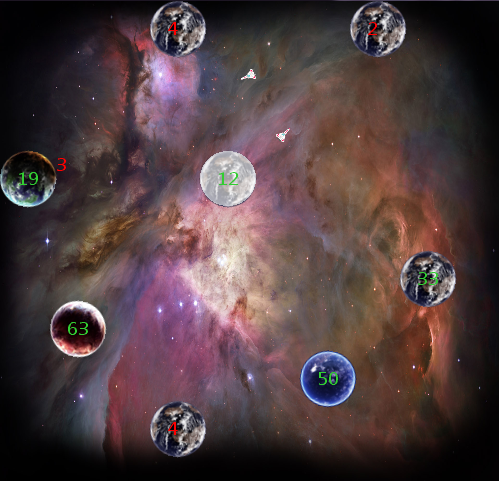
\includegraphics[scale=0.7]{RTS.png}
\caption{Frame rate as a function of numbers of entities.}
\label{fps_chart}
\end{figure} 


%conclusions
%% Changed by PS, April 4, 2014.

\section{Future work}
\label{sec:future_work}
The Casanova 2 language is capable of implementing usable and quite complex games. The language, while usable, is currently still in development as it misses a few features. In particular, support for multiplayer games is at this moment lacking. We believe that the existing mechanisms for handling time offered by Casanova 2 could be augmented with relatively little effort in order to greatly simplify the hard task of building multiplayer games. This is part of future work, that we are currently engaging in. We are also doing usability studies using students from various disciplines and backgrounds.

The high level view of the game that the Casanova 2 compiler provides can be exploited in order to improve the programmer experience. This means that we could use tools for code analysis (such as abstract interpretation \cite{nielson1999principles} or type system extensions) in order to better understand the game being built, and to help with correctness analysis, performance analysis, or even optimization.


%\subsection{User study}
%We wish to perform an in-depth user study for Casanova 2 to improve usability in the development process. We have already performed a partial (and quite promising) small user study which we will extend and complete.


%We have performed the following test: we gathered a group of students of game programming and a group of students of game design. We gave them a series of Casanova 2 samples, printed on paper. Each student had to guess the functionality of each sample, and sketch a screen-shot. Furthermore, each student also provided some additional feedback on the language.

%The samples were: (\textit{i}) a string of text moved around the screen with the keyboard, (\textit{ii}) a string of text that moves along a predefined path automatically, and (\textit{iii}) an asteroid shooter.

%Eleven (over a total of thirteen) students understood the samples completely, both drawing the screen-shots and explaining the dynamics of the game correctly. Two students were lost on the syntactic differences between Casanova 2 and the more familiar C-like syntax. The direct feedback was mostly centred around a series of common observations, which are reported in Table \ref{students_feedback}. For each observation, the table reports how many times we encountered it.

%\begin{table}[!t]
%% increase table row spacing, adjust to taste
%\renewcommand{\arraystretch}{1.3}
% if using array.sty, it might be a good idea to tweak the value of
% \extrarowheight as needed to properly center the text within the cells

%\caption{Feedback from students}
%\label{students_feedback}
%\centering

%% Some packages, such as MDW tools, offer better commands for making tables
%% than the plain LaTeX2e tabular which is used here.
%\begin{tabular}{|c||c|}
%\hline
%Syntax is unfamiliar at first & 3\\
%\hline
%Syntax is clear & 8\\
%\hline
%Indentation instead of parentheses is a downside & 2\\
%\hline
%List processing with queries is very effective & 1\\
%\hline
%Rules are a good abstraction for games & 2\\
%\hline
%\end{tabular}
%\end{table}

%We also built a significantly bigger sample, which we asked only three students to study. The sample is a checkpoint-based RTS (see Figure \ref{RTS game} for a screenshot). All students correctly identified the game mechanics, and provided some additional feedback. Most of this feedback overlaps with that obtained for the samples, but some new observations emerge. Arguably, some patterns become visible only with larger samples:
%\begin{itemize}
%\item \texttt{wait} and \texttt{when} are very powerful
%\item Multiple rules on the same field are very powerful
%\item Multiple rules on the same field may lead to behaviours that are complex to understand
%\end{itemize}


\section{Conclusions}
\label{sec:conclusions}

Casanova 2, a language specifically designed for building computer games, may offer a solution for the high development costs of games. The goal of Casanova 2 is to reduce the effort and complexities associated with building games. Casanova 2 manages the game world through entities and rules, and offers constructs (wait and yield) to deal with the run-time dynamics. As shown by the benchmarks in Section \ref{sec:evaluation}, we believe that we have taken a significant step towards reaching these goals. In fact, we achieved at the same time very good performance and simplicity, thereby empowering developers with limited resources. 

\bibliographystyle{abbrv}
\bibliography{Sections/References}
\end{document}
